% bei Standalone in documentclass noch:
% \RequirePackage{luatex85}

\documentclass[captions=tableheading, titlepage= firstiscover, parskip = half , bibliography=totoc]{scrartcl}
%paper = a5 für andere optinen
% titlepage= firstiscover
% bibliography=totoc für bibdateien
% parskip=half  Veränderung um Absätze zu verbessern

\usepackage{scrhack} % nach \documentclass
\usepackage[aux]{rerunfilecheck}
\usepackage{polyglossia}
\usepackage[style=numeric, backend=biber]{biblatex} % mit [style = alphabetic oder numeric] nach polyglossia
\addbibresource{lit.bib}
\setmainlanguage{german}

\usepackage[autostyle]{csquotes}
\usepackage{amsmath} % unverzichtbare Mathe-Befehle
\usepackage{amssymb} % viele Mathe-Symbole
\usepackage{mathtools} % Erweiterungen für amsmath
\usepackage{fontspec} % nach amssymb
% muss ins document: \usefonttheme{professionalfonts} % für Beamer Präsentationen
\usepackage{longtable}

\usepackage[
math-style=ISO,    % \
bold-style=ISO,    % |
sans-style=italic, % | ISO-Standard folgen
nabla=upright,     % |
partial=upright,   % /
]{unicode-math} % "Does exactly what it says on the tin."
\setmathfont{Latin Modern Math}
% \setmathfont{Tex Gyre Pagella Math} % alternativ

\usepackage[
% die folgenden 3 nur einschalten bei documenten
locale=DE,
separate-uncertainty=true, % Immer Fehler mit ±
per-mode=symbol-or-fraction, % m/s im Text, sonst \frac
]{siunitx}

% alternativ:
% per-mode=reciprocal, % m s^{-1}
% output-decimal-marker=., % . statt , für Dezimalzahlen

\usepackage[
version=4,
math-greek=default,
text-greek=default,
]{mhchem}

\usepackage[section, below]{placeins}
\usepackage{caption} % Captions schöner machen
\usepackage{graphicx}
\usepackage{grffile}
\usepackage{subcaption}

% \usepackage{showframe} Wenn man die Ramen sehen will

\usepackage{float}
\floatplacement{figure}{htbp}
\floatplacement{table}{htbp}

\usepackage{mhchem} %chemische Symbole Beispiel: \ce{^{227}_{90}Th+}


\usepackage{booktabs}

 \usepackage{microtype}
 \usepackage{xfrac}

 \usepackage{expl3}
 \usepackage{xparse}

 % \ExplSyntaxOn
 % \NewDocumentComman \I {}  %Befehl\I definieren, keine Argumente
 % {
 %    \symup{i}              %Ergebnis von \I
 % }
 % \ExplSyntaxOff

 \usepackage{pdflscape}
 \usepackage{mleftright}

 % Mit dem mathtools-Befehl \DeclarePairedDelimiter können Befehle erzeugen werden,
 % die Symbole um Ausdrücke setzen.
 % \DeclarePairedDelimiter{\abs}{\lvert}{\rvert}
 % \DeclarePairedDelimiter{\norm}{\lVert}{\rVert}
 % in Mathe:
 %\abs{x} \abs*{\frac{1}{x}}
 %\norm{\symbf{y}}

 % Für Physik IV und Quantenmechanik
 \DeclarePairedDelimiter{\bra}{\langle}{\rvert}
 \DeclarePairedDelimiter{\ket}{\lvert}{\rangle}
 % <name> <#arguments> <left> <right> <body>
 \DeclarePairedDelimiterX{\braket}[2]{\langle}{\rangle}{
 #1 \delimsize| #2
 }

\setlength{\delimitershortfall}{-1sp}

 \usepackage{tikz}
 \usepackage{tikz-feynman}

 \usepackage{csvsimple}
 % Tabellen mit \csvautobooktabular{"file"}
 % muss in table umgebung gesetzt werden


% \multicolumn{#Spalten}{Ausrichtung}{Inhalt}

\usepackage{hyperref}
\usepackage{bookmark}
\usepackage[shortcuts]{extdash} %nach hyperref, bookmark

\newcommand{\ua}[1]{_\symup{#1}}
\newcommand{\su}[1]{\symup{#1}}


\title{Versuch 356}
\subtitle{Kettenschaltung mit LC-Gliedern}
\author{Sebastian Pape\\
        sepa@gmx.de \and
        Jonah Nitschke\\
        lejonah@web.de}
\date{Durchführung: 17.01.2017\\
      Abgabe: 24.01.2017}

\begin{document}
\maketitle

\section{Einleitung}

In dem folgenden Versuch geht es um die Betrachtung von Wellen mithilfe eines
Schwingkreises als Analogon zum verketteten harmonischen Oszillators in der
Mechanik. Dabei werden verschiedene charakteristische Größen der entstehenden
stehenden Wellen betrachtet, wie zum Beispiel Dispersionsrelation sowie Phasenverschub
zwischen der eingehenden und ausgehenden Spannung.

\section{Theorie}

\subsection{Die Dispersionsrelationen}

Im allgemeinen gibt die Dispersionsrelation an, in wie weit verschiedene physikalische
Größen Abhängigkeiten von der Frequenz aufweisen. Um diese Abhängigkeiten für
eine LC-Kettenschaltung zu bestimmen, wird zunächst mithilfe der Kirchoffschen
Regeln die Schwingungsgleichung hergeleitet und auf n Kettenglieder verallgemeinert.
Mit der Annahme, dass alle Kettenglieder mit der gleichen Frequenz $\omega$ schwingen
und lediglich beim Durchlaufen einen Phasenverschub $\theta$ erfahren, lässt sich
für die Kette folgende Dispersionsrelation herleiten:

\begin{equation}
  \omega^2 = \frac{2}{LC}(1-\cos{\theta}) .
  \label{eqn:RelationC}
\end{equation}

Aus dieser Formel lässt sich also die Phasenänderung pro Kettenglied in Abhängigkeit
der angelegten Frequenz bestimmen.

Die bei Formel \eqref{eqn:RelationC} bestimmte Dispersionsrelation lässt
sich etwas verallgemeinern, indem eine Kettenschaltung  mit alternierend eingebauten
Kondensatoren $C\ua{1}$ und $C\ua{2}$ verwendet wird. Bei der Lösung der analog
zu der obigen Schaltung bestimmten Schwingungsgleichung wird hierbei die Annahme
getroffen, dass alle Kettenglieder immernoch mit der gleichen Frequenz schwingen,
allerdings jedes zweite Kettenglied eine andere Amplitude aufweist. Somit ergibt
sich für die $LC\ua{1}C\ua{2}$-Kette folgende Dispersionsrelation:

\begin{equation}
  \omega\ua{1,2}^2 = \frac{1}{L} \left\{ \frac{1}{C\ua{1}} + \frac{1}{C\ua{1}}
  \right\} \, \pm \, \frac{1}{L} \sqrt{ \left\{ \frac{1}{C\ua{1}} + \frac{1}{C\ua{1}}
  \right\}^2  - \frac{4\cos(\theta)^2}{C\ua{1}C\ua{2}}} .
  \label{eqn:RelationC1C2}
\end{equation}

\begin{figure}
  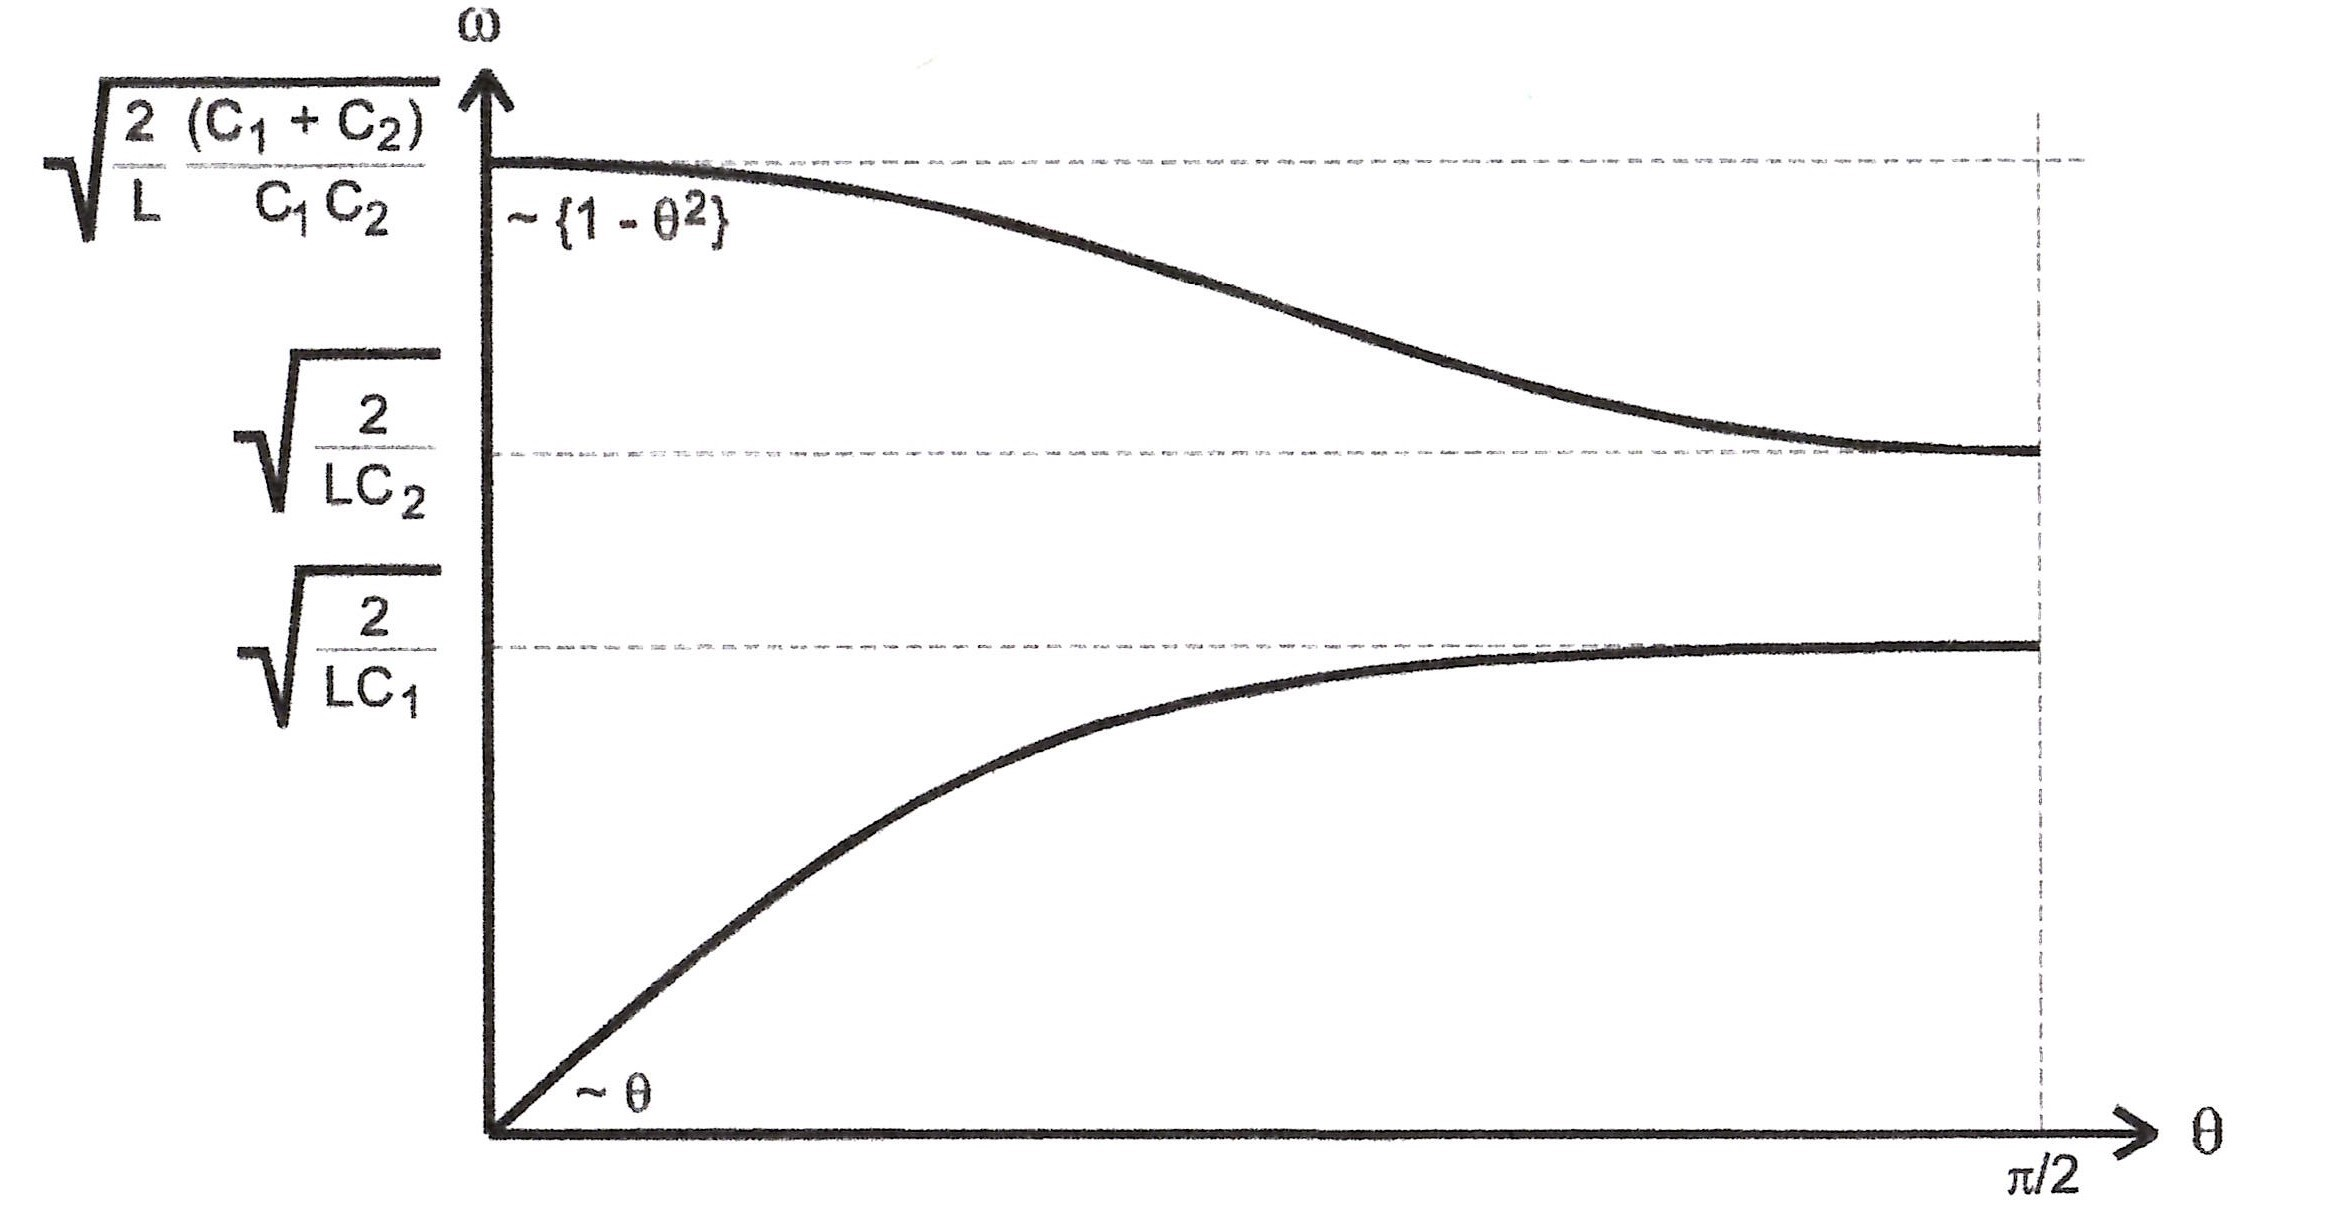
\includegraphics[width = \textwidth]{DIspersionskurveC1C2.jpg}
  \caption{Dispersionskurve bei einer Kette mit zwei unterschiedlichen Kondensatoren}
  \label{fig:RelationC12}
\end{figure}

Wie der Formel \eqref{eqn:RelationC1C2} entnommen werden kann, bilden sich bei
dieser Dispersionsrelation zwei Äste, auch akustischer und optische Ast genannt
(siehe Abbildung \ref{fig:RelationC12}). Zwischen den beiden Ästen existiert ein Bereich, welcher
bei der Schwingung nicht auftretenden Frequenzen beinhält. Während $\omega\ua{1}$
bei $\theta = \frac{\pi}{2}$ ein Maximum besitzt, tritt dort für $\omega\ua{2}$
ein Minimum auf (siehe Abbildung \ref{fig:RelationC12}).


\begin{align}
  \omega\ua{1} &= \sqrt{ \frac{1}{L} \frac{2(C\ua{1} + C\ua{2})}{C\ua{1}C\ua{2}}} \,
  \left\{ 1 - \theta^2 \frac{C\ua{1}C\ua{2}}{(C\ua{1} + C\ua{2})^2} \right\} \\
  \omega\ua{2} &= \sqrt{ \frac{2}{L(C\ua{1} + C\ua{2})}} \, \theta
\end{align}

Aus den bestimmten Dispersionsrelationen lassen sich nun ebenfalls die Phasen- und
die Gruppengeschwindigkeit herleiten. Da die Gruppenheschwindigkeit in dem Versuch
jedoch nicht betrachtet wird, wird im folgenden nur auf die Phasengeschwindigkeit
eingegangen:

\begin{equation}
  v\ua{Ph} = \frac{\omega}{\theta} = \frac{\omega}{\arccos(-\frac{1}{2}\omega^2LC)}
\end{equation}

Die Dispersion verschwindet in dem Bereich kleiner Frequenzen, also bei $\omega$
<< 1/LC. Beim Erreichen der Grenzfrequenz $\omega\ua{G}$ = 2/$\sqrt{\su{LC}}$ erreicht
die Phasengeschwindigkeit einen Minimalwert:

\begin{equation}
  v\ua{Ph\ua{min}} =  \frac{2}{\pi} \frac{1}{\sqrt{\su{LC}}}
\end{equation}

\subsection{(Undendlich lange) LC-Ketten}

Interessant für die Schltungstechnik ist auch der am Eingang der Kette gemessene
Eingangswiderstand, welcher als Quotient von der am Eingangskondensator anliegenden
Spannung $U\ua{0}$ und dem in die Schaltung hineinfließenden Strom $I\ua{0}$
definiert ist:

\begin{equation}
  Z(\omega) = \frac{U\ua{0}}{I\ua{0}} = \sqrt{ \frac{L}{C}} \frac{1}{ \sqrt{1 - \frac{1}{4} \omega^2 LC} }.
\end{equation}

Der Eingangswiderstand einer (undendlich langen) Kette ist somit rein reell,
obwohl in der Schaltung nur Komponenten mit imaginären Impedanzen verwendet wurden.
Dieses Ergebnis ist auch zu erwarten gewesen, da in einer (undendlich langen) Kette
keine Reflexion auftreten sollte. Somit sind Strom und Spannung an jedem Ort in
Phase, elektrische Energie kann lediglich in die Kette hineinfließen und eine
(unendlich lange) Kette kann also auch bei einer begrenzten mit dem Wellenwiderstand
als Abschlusswiderstand simuliert werden.

\begin{figure}
  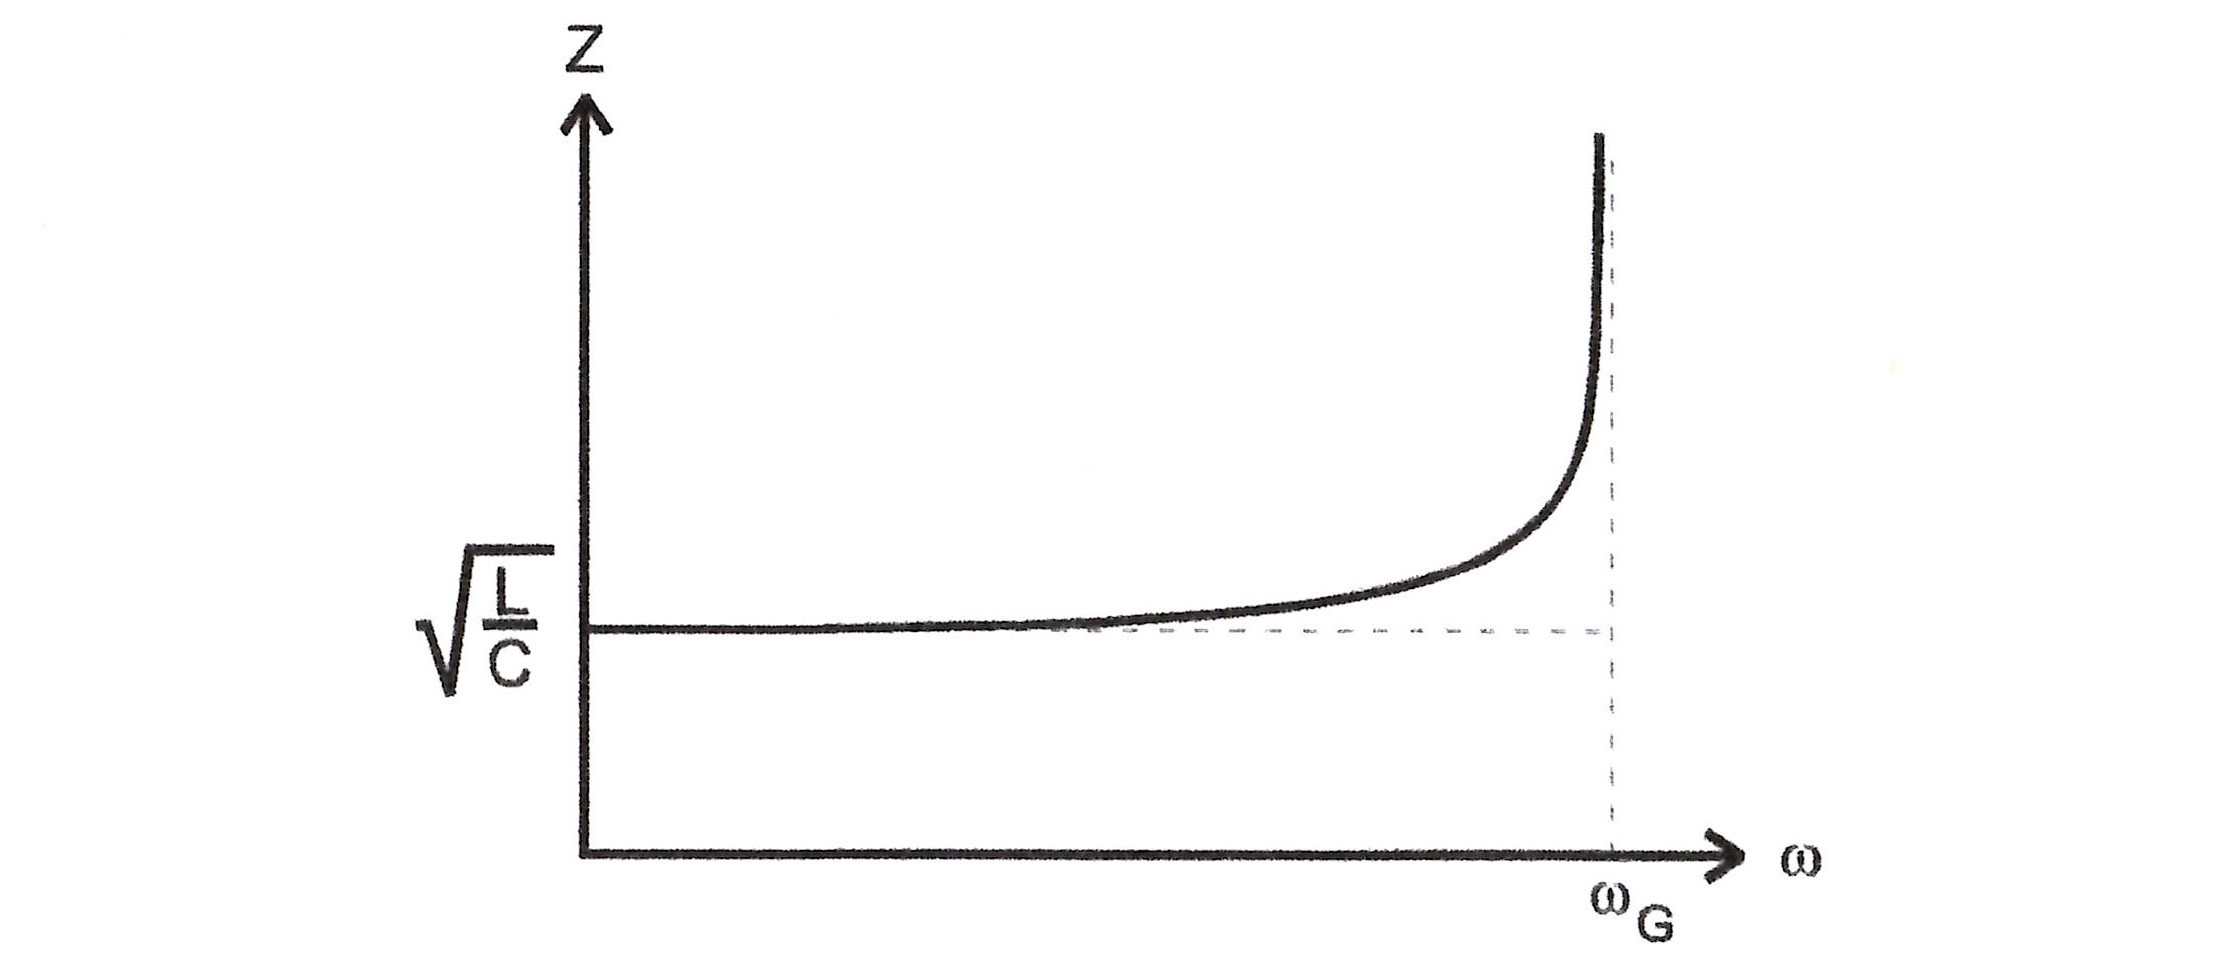
\includegraphics[width = \textwidth]{AbhaengigkeitImpedanz.jpg}
  \caption{Frequenzabhängigkeit der Impedanz}
  \label{fig:Impedanzabhängigkeit}
\end{figure}

In Abbildung \ref{fig:Impedanzabhängigkeit} sieht man die Abhängigkeit der Impedanz
von der angelegten Frequenz.
Über den angeschlossenen Widerstand und den Wellenwiderstand lässt sich das
Verhältnis zwischen Amplitude der eingehenden und reflektierten Spannung über folgende
Formel bestimmen:

\begin{equation}
  \frac{U\ua{ref}}{U\ua{E}} = \frac{r - Z}{r + Z}.
\end{equation}


Die Welle weißt nun für verschieden Abschlusswiderstände unterschiedliche
Eigenschaften auf, die im folgenden aufgelistet sind:


\renewcommand{\labelenumi}{\alph{enumi})}
\begin{enumerate}
  \item offenes Ende (R = $\infty$): \\
        $U\ua{ref}$ = $U\ua{E}$ $\implies$ vollständige Reflexion ohne Phasensprung.

  \item kurzgeschlossene Kette (R = 0): \\
        $U\ua{ref}$ = - $U\ua{E}$ $\implies$ vollständige Reflexion mit Phasensprung.

  \item Abschluss mit Wellenwiderstand (R = Z): \\
        $U\ua{ref}$ = 0 $\implies$ keine Reflexion.

  \item in allen anderen Fällen tritt eine Teilreflexion auf und bei einem nicht
        reelen R zusätzlich eine Phasendrehung.
\end{enumerate}

Bei den ersten beiden Fällen tritt also durch Überlagerung einer hinlaufenden
Welle und der rücklaufenden Welle eine Überlagerung zu einer stehenden Welle
statt. Dabei entstehen Schwingungsknoten, an denen die Amplitude für alle
Zeiten verschwindet:

\begin{align}
  n\ua{z}\theta &= z \frac{\pi}{2} \, \, \, \, \, (z = 1,3,5, ...)
  \label{eqn:offenesEnde}
\end{align}

\begin{align}
  n\ua{z}\theta &= z \pi \, \, \, \, \, (z = 1,2,3, ...)
  \label{eqn:geschlossenesEnde}
\end{align}

Dabei bezieht sich die Formel \eqref{eqn:offenesEnde} auf ein offenes Ende und
die Formel \eqref{eqn:geschlossenesEnde} auf ein geschlossenes Ende.

Im Fall $R = \infty$ kann sich allerdings nur dann eine stehende Welle ausbilden,
wenn am Kettenende (n=$\su{n}\ua{max}$) ein Spannungsbauch befindet.

\newpage

\section{Versuchsdurchführung}

\subsection{Bestimmung der Durchlasskurve}

\begin{figure}
  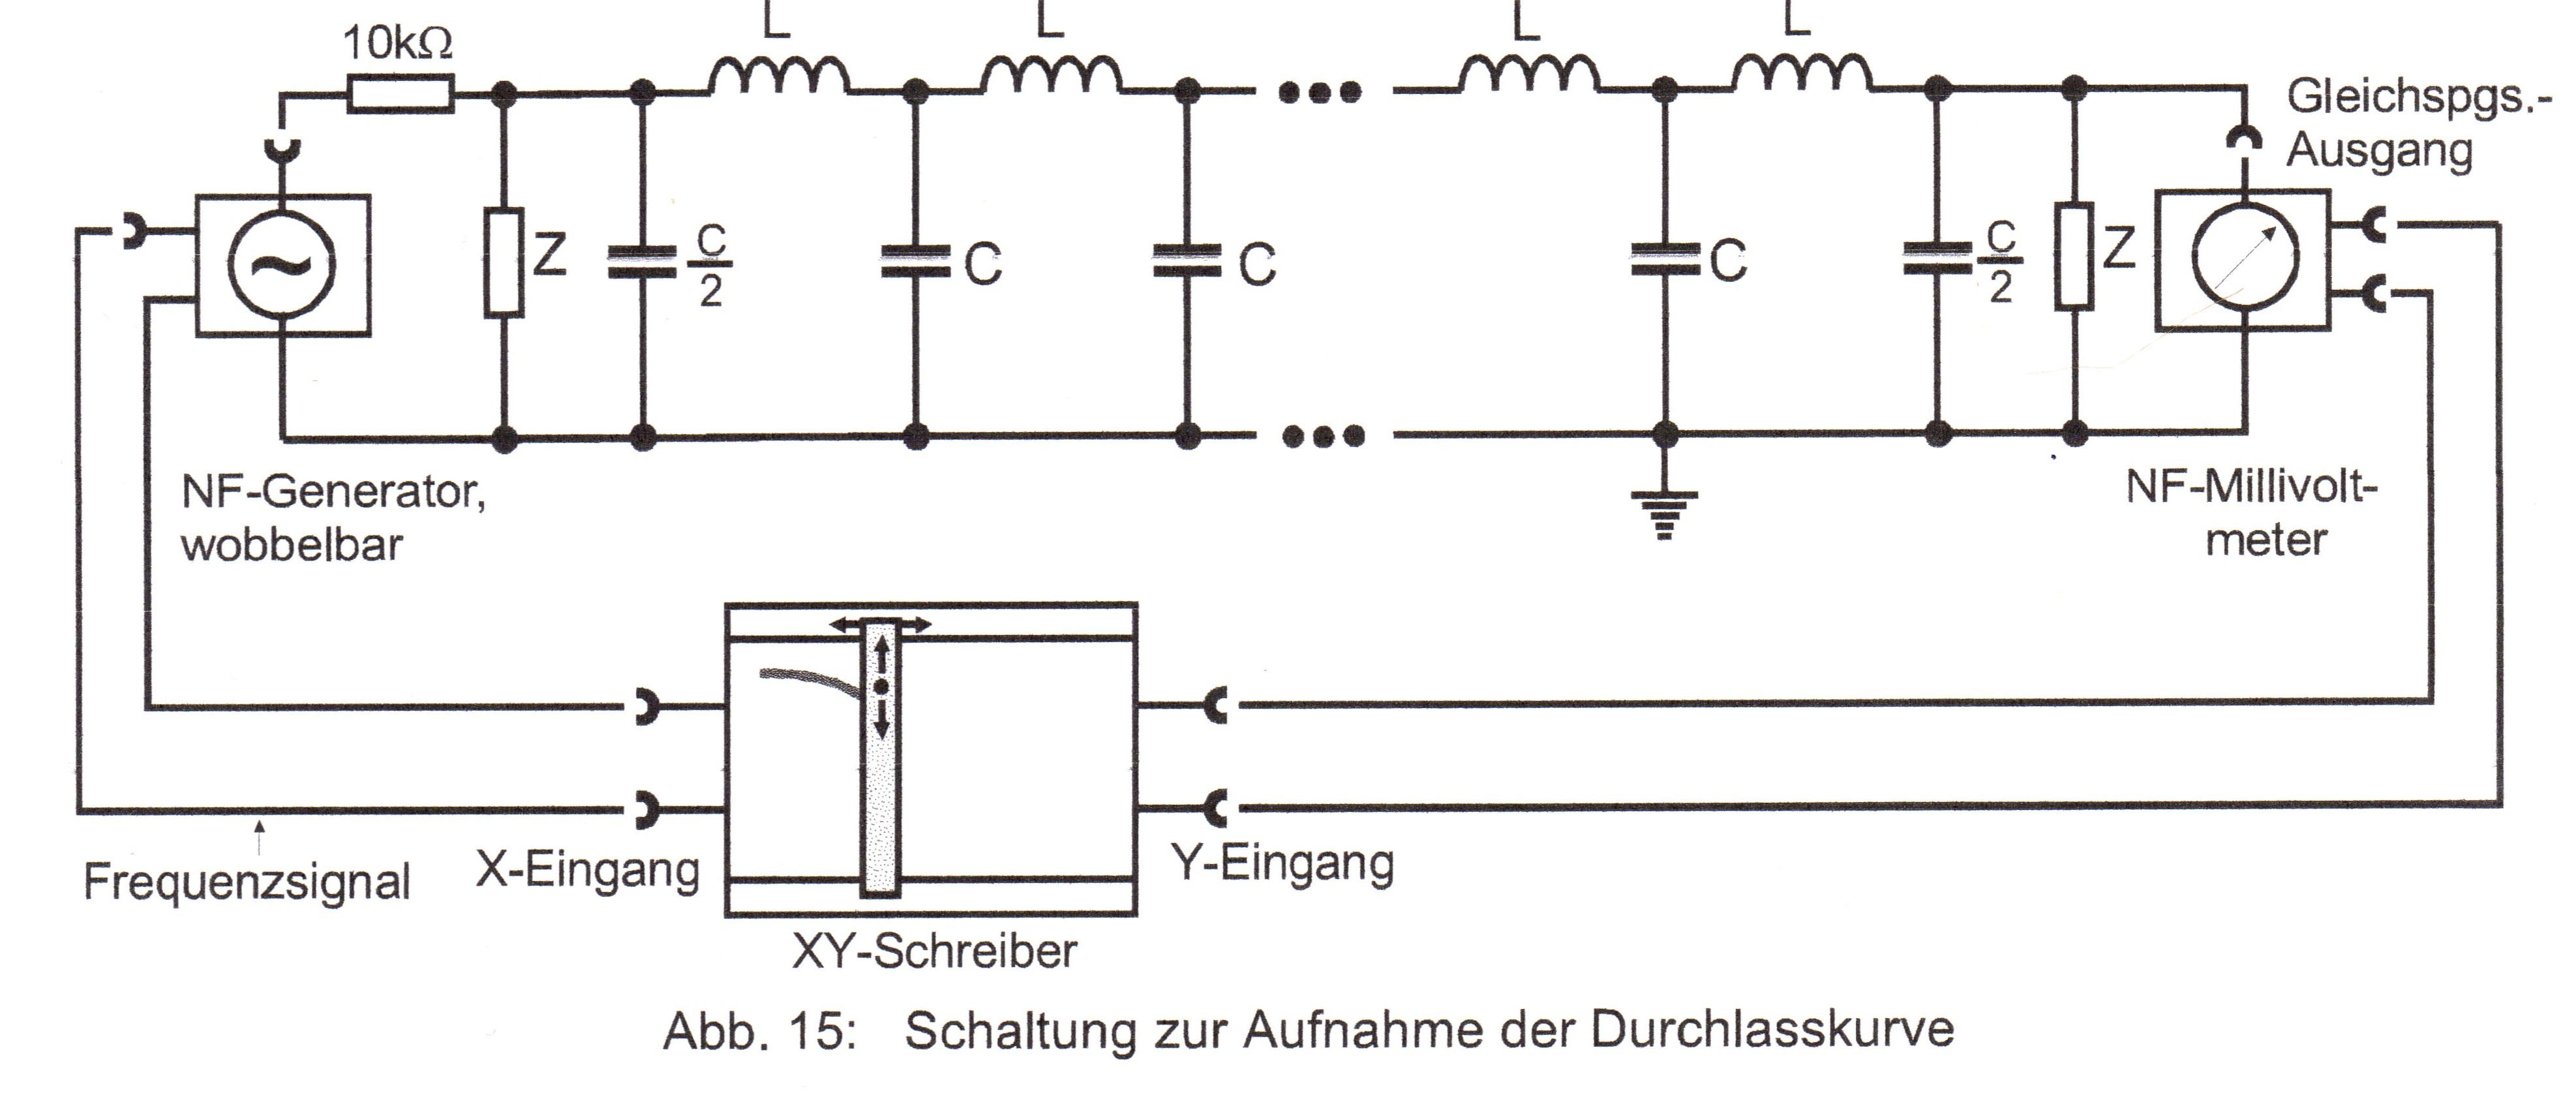
\includegraphics[width = \textwidth]{Durchlasskurve.jpg}
  \caption{Schaltung zur Bestimmung der Durchlasskurve und dem Nachweis stehender Wellen}
  \label{fig:Durchlasskurve}
\end{figure}

In dem ersten Teil des Experimentes wird mithilfe eines Schreibers eine Durchlasskurve
für beide Ketten angefertigt. Dabei wird an dem Generator ein Sweep eingestellt,
sodass der Schreiber die gemessenen Spannung am Ausgang der LC-Kette in Abhängigkeit
der anliegenden Frequenz aufzeichnet. Dabei müssen die Achsen so angepasst sein,
dass die Grenzfrequenzen auf der angefertigten Zeichnung ebenfalls zu sehen sind.
Die Schaltung für diesen Teil der Messung ist in Abbildung \ref{fig:Durchlasskurve} zu sehen.


\subsection{Bestimmung der Dispersionsrelation}

\begin{figure}
  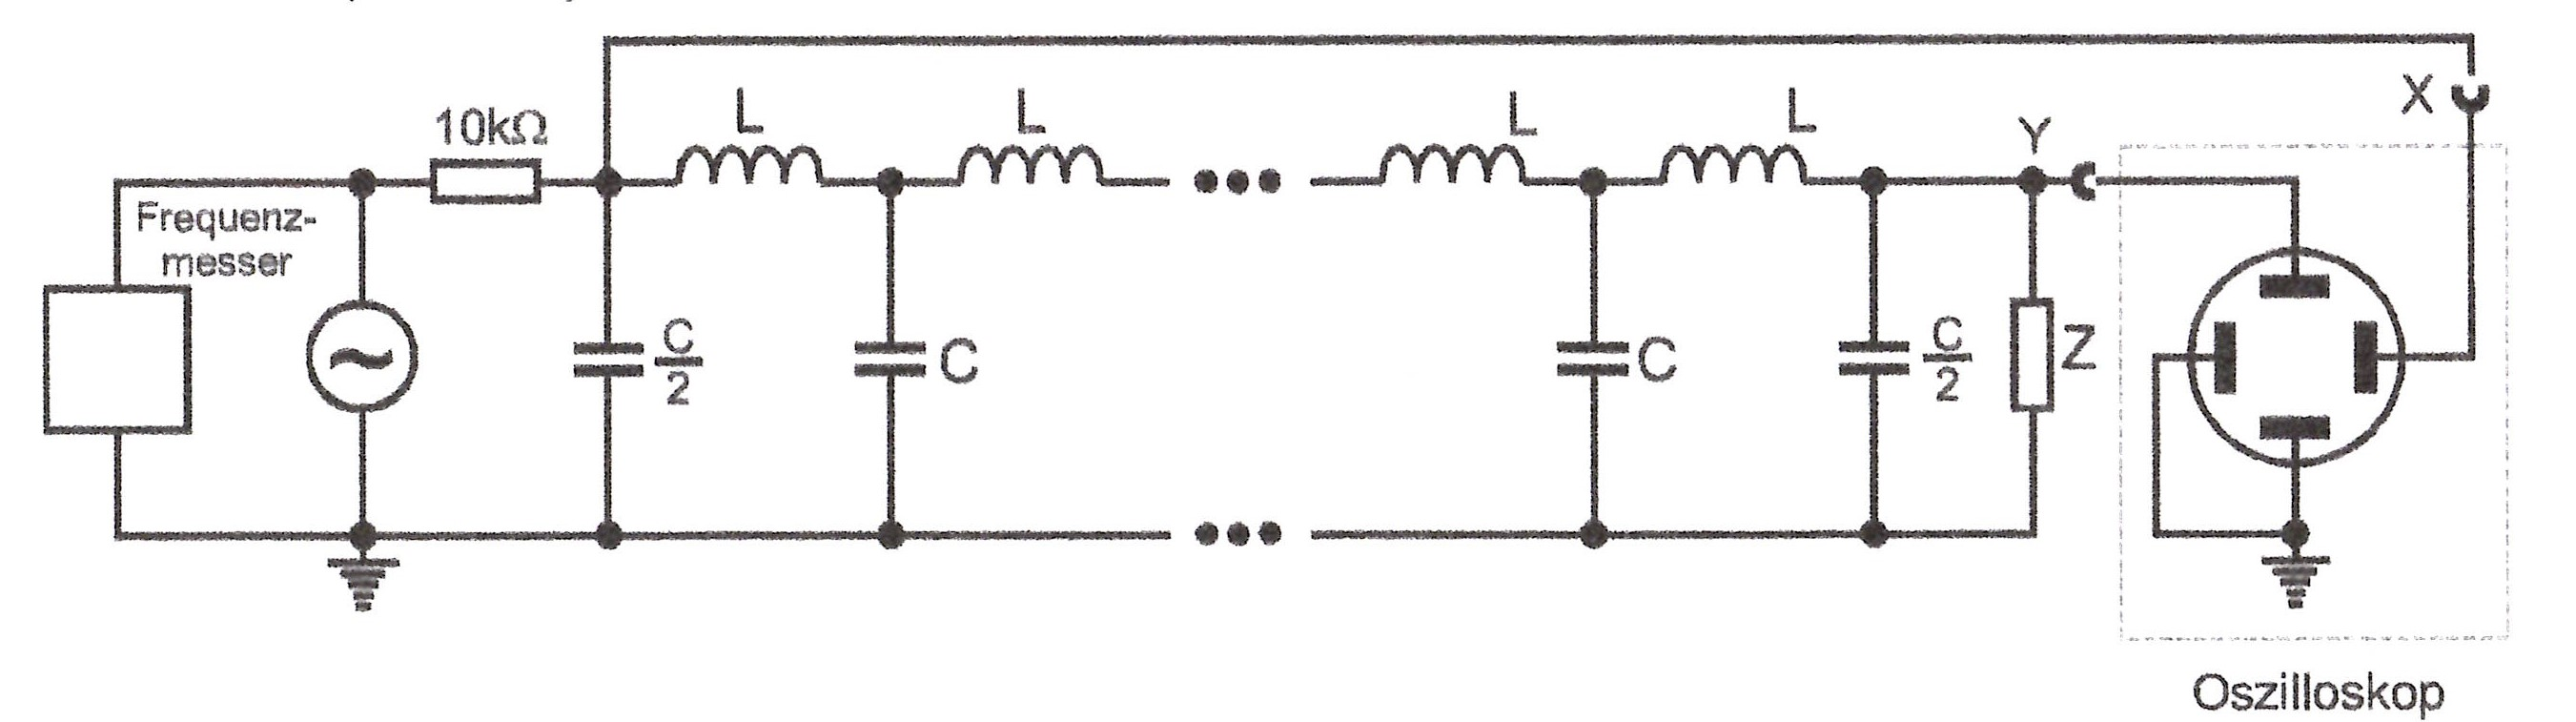
\includegraphics[width = \textwidth]{Dispersionsrelation.jpg}
  \caption{Schaltung zur Bestimmung der Dispersionsrelation}
  \label{fig:Dispersion}
\end{figure}

Mithilfe der in Abbildung \ref{fig:Dispersion} dargestellten Schaltung lässt sich die Phasenverschiebung
pro Kettenglied betrachten. Dafür wird an einem Oszillloskop mithilfe von Lissajous-Figuren
die Phasenverschiebung zwischen Eingangs- und Ausgangsspannung betrachtet, wobei
lediglich Frequenzen mit einer Phasenverschiebung eines Vielfachen von $\pi$
notiert werden.


\subsection{Nachweis von stehenden Wellen}

Mit der Schaltung nach Abbildung \ref{fig:Durchlasskurve} (ohne Schreiber und Wobbeleinrichtung) wird
nun versucht, stehende Wellen nachzuweisen.
Dafür wird mit einem Millivoltmeter anfangs die Ausgangsspannung gemessen, um eine
Frequenz mit einem Spannungsmaximum am Kettenende zu finden. Dach wird an jedem
Kettenglied die auftretende Spannung gemessen. Diese Messung wird für eine
beiderseits offene Kette mit der 1. und 2. Eigenschwingung durchgeführt und danach
für eine mit dem Wellenwiderstand als Abschlusswiderstand eingestellte Kette
für eine beliebige Frequenz wiederholt.



\end{document}
